\subsection{Building blocks}%
\label{BuildingBlocks}

\paragraph*{Hybrid encryption}\label{KEM}

\Iac{HE} scheme is a combination of \iac{PKE} scheme and \iac{SKE} scheme.
The \ac{PKE} scheme is used as \iac{KEM} to encrypt a symmetric key for the 
\ac{SKE} scheme.
Then the \ac{SKE} scheme is used as \iac{DEM} to encrypt the actual data.

Whenever we use \iac{PKE} scheme, we mean to employ it in \iac{HE} scheme.

\paragraph*{\Acl*{BE}}\label{BE}

\begin{figure}[t]
\centering
  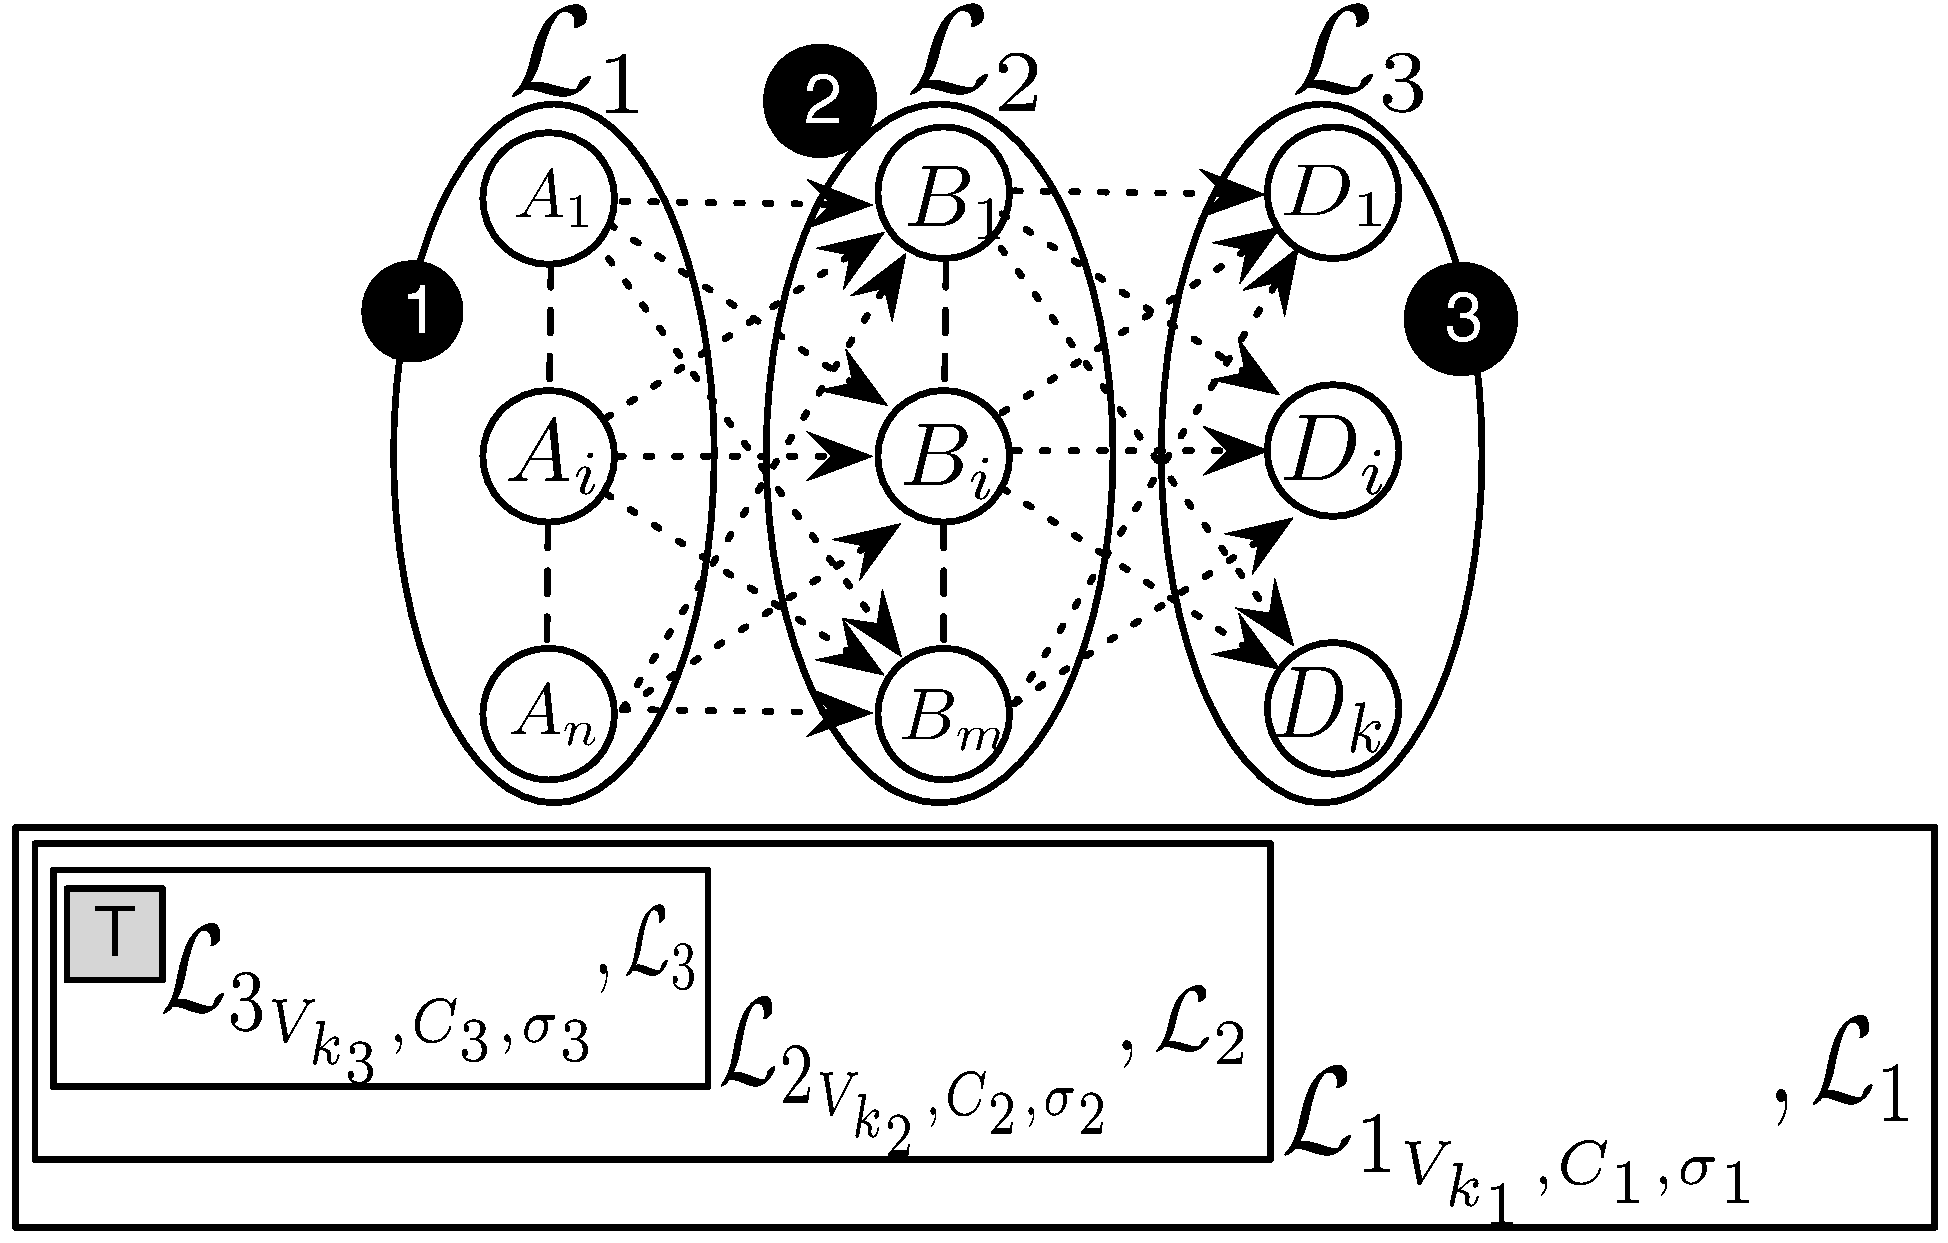
\includegraphics[scale=.20]{figures/pors2.pdf}
  \caption{\label{fig:por} Group Onion Routing}
\end{figure}

Figure~\ref{fig:por},\ding{182}, \ding{183}, \ding{184}).
We will do onion routing with many alternative nodes per hop.
This means that we encrypt the same message for more than one possible 
recipient.
Given this, it is natural to look for a suitable \ac{BE} scheme.
More specifically, we are interested in \iac{BE} scheme adapted for \iac{P2P} 
setting, where devices can dynamically join and leave --- \ie we do not want too 
much cost for joining or leaving, \eg from key regeneration.
We also want some privacy properties, \eg those of \ac{ANOBE}.

Our \ac{P2P} setting requires something similar to \iac{DBE} scheme.
However, we want a slightly different definition.
We say that \iac{BE} scheme is \iac{DeBE} if
\begin{enumerate}
  \item the setup is independent from the expected number of users or an upper 
    bound thereof,
  \item a new user can join at any time and the already issued decryption keys 
    can remain the same,
  \item the previous (public) encryption key can still be used if the newly 
    joined user is not in the recipient set.
\end{enumerate}
Unlike the definition of \textcite{DynamicBroadcastEncryption}, we desire 
forward secrecy --- in our scenario it makes no sense that new devices can 
decrypt old ciphertexts.
We also want to change the restriction on the ciphertext size:
whereas \textcite{DynamicBroadcastEncryption} require the ciphertext size to be 
independent from the expected number of users, we want it to be independent of 
the total number of users --- \ie it can depend on the recipient set.
In this sense, the trivial \ac{BE} scheme would fulfil our definition, but not 
the definition of dynamic~\cite{DynamicBroadcastEncryption}.

\NewScheme{\ANOBE}{ANOBE}
\NewScheme{\DeBE}{DeBE}
\NewAlgorithm{\DeBEsetup}{\DeBE[Setup]}
\NewAlgorithm{\DeBEjoin}{\DeBE[Join]}
\NewAlgorithm{\DeBEenc}{\DeBE[Enc]}
\NewAlgorithm{\DeBEdec}{\DeBE[Dec]}

Our \ac{DeBE} scheme, \(\DeBE\), provides the following algorithms:
\(\DeBEsetup, \allowbreak \DeBEjoin, \allowbreak \DeBEenc, \allowbreak 
  \DeBEdec\).
We will use the proposed instantiation of \iac{ANOBE} scheme by \textcite{ANOBE} 
to instantiate our \ac{DeBE} scheme.
We will simply divide the steps of the \(\ANOBE\) algorithms differently.

\NewVariable{\mpk}{MPK}
\NewScheme{\Enc}{E}
\NewScheme{\Sign}{S}

\(\DeBEsetup[\lambda]\): takes the security parameter \(\lambda\) and generates 
the global parameters for the underlying IND-CCA encryption scheme \(\Enc\) and 
the one-time signature scheme \(\Sign\).
It also creates a master public key, \(\mpk = \emptyset\).

\NewVariable{\pk}{pk}
\NewVariable{\sk}{sk}

\((\pk_i, \sk_i)\gets \DeBEjoin[i]\): generates the public--private key-pair 
\((\pk_i, \sk_i)\) for device \(i\) when it joins.
It also adds \(\pk_i\) to \(\mpk\).
See \cref{DeBEsetup} for an algorithmic overview.

\begin{figure}
  \framebox{\begin{minipage}{0.96\linewidth}
  \begin{algorithmic}
    \Require{$\Enc$ is an IND-CCA \ac{PKE} scheme, $\Sign$ is a one-time 
      signature scheme.}

    \Function{\DeBEsetup}{$\lambda$}
      \State $\Enc[Setup](\lambda), \Sign[Setup](\lambda)$
      \State $\mpk\gets \emptyset$
    \EndFunction

    \Function{\DeBEjoin}{$i$}
      \State $(\pk_i, \sk_i)\gets \Enc[Keygen]$
      \State $\mpk\gets \mpk\cup \{\pk_i\}$
      \State \Return $(\pk_i, \sk_i)$
    \EndFunction
  \end{algorithmic}
  \end{minipage}}
  \caption{\label{DeBEsetup}\label{DeBEjoin}%
    Algorithmic overview of \(\DeBEsetup\) and \(\DeBEjoin\).
  }
\end{figure}

\NewVariable{\ssk}{ssk}
\NewVariable{\vk}{vk}

\((\vk, C, \sigma)\gets \DeBEenc[\mpk, S, m]\):
takes a message \(m\) and a recipient set \(S\), it then encrypts the message 
for each recipient's key, signs the tuple of all ciphertexts and returns the 
verification key, ciphertexts and signature.
(Note that the signature does not authenticate the sender, it ties the 
ciphertext together and is needed for correctness, we refer to~\cite{ANOBE} for 
details.)

\(m\gets \DeBEdec[\mpk, \sk_i, (\vk, C, \sigma)]\):
takes a ciphertext \((\vk, C, \sigma)\) and tries to decrypt the sub-ciphertexts 
in \(C\) using the private key \(\sk_i\).
If one succeeds, that message is returned, otherwise \(\bot\) is returned on 
failure.
This trial-and-error decryption is costly as it makes the decryption function 
complexity \(O(|S|)\).
\textcite{ANOBE} also presented a tag-hint system along with their \ac{ANOBE} 
scheme.
The tag-hint system reduced the complexity back to \(O(1)\).
As this is not relevant for our discussion, we refer the reader to~\cite{ANOBE} 
but note that it can be used.

Both \(\DeBEenc\) and \(\DeBEdec\) are the same as in~\cite{ANOBE}.
The algorithms are illustrated in \cref{DeBEenc,DeBEdec}.

\begin{figure}
  \framebox{\begin{minipage}{0.96\linewidth}
  \begin{algorithmic}
    \Require{$\Enc$ is an IND-CCA \ac{PKE} scheme, $\Sign$ is a one-time 
      signature scheme.}

    \Function{$\DeBEenc$}{$\mpk, S, m$}
      \State $(\ssk, \vk)\gets \Sign[Keygen]$
      \State Choose a random permutation \(\pi\colon S\to S\).
      \For{$i \in S$}
        \State $c_i\gets \Enc[Enc](\pk_i, m\concat \vk)$
      \EndFor
      \State $C\gets ( c_{\pi(1)}, \dotsc, c_{\pi(|S|)} )$
      \State $\sigma\gets \Sign[Sign](\ssk, C)$
      \State \Return $(\vk, C, \sigma)$
    \EndFunction

    \Function{$\DeBEdec$}{$\mpk, \sk_i, (\vk, C, \sigma)$}
      \If{$\Sign[Verify](\vk, C, \sigma) = \bot$}
        \State \Return $\bot$
      \EndIf
      \For{$c\in C$}
        \Comment Trial-and-error decryption
        \State $M\gets{\Enc[Dec](\sk_i, c)}$
        \If{$M = \bot$}
          \State \Return $\bot$
        \ElsIf{$M = (m, \vk)$}
          \State \Return $m$
        \EndIf
      \EndFor
      \State \Return $\bot$
    \EndFunction
  \end{algorithmic}
  \end{minipage}}
  \caption{\label{DeBEenc}\label{DeBEdec}%
    An algorithmic overview of the encryption and decryption algorithms in the 
    \(\DeBE\) scheme, identical to those of \(\ANOBE\).%
  }
\end{figure}

